\chapter{Simulation Testing}
\section{Bucket of water}

\begin{figure}[H]
  \centering
    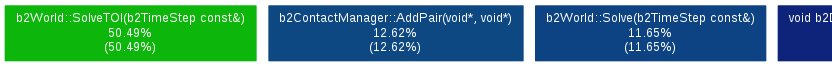
\includegraphics[scale=0.4]{project/images/infi_water.png}
  \caption{\textbf{call graph for water of very small size}}
\end{figure}

\paragraph{
The above is the call graph when we tried to implement bucket and water.
we made the size of water articles very small and made  the number of particles very large ,because of which the solveTOI function took very large time .we resolved it by increasing the size and reducing the number of particles.
the final call graph is as below.
}

\begin{figure}[H]
  \centering
    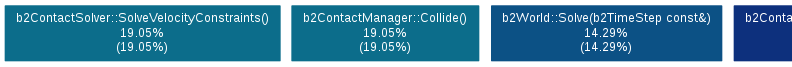
\includegraphics[scale=0.4]{project/images/normal_water.png}
  \caption{\textbf{call graph for final bucker and water}}
\end{figure}



We also generated and analysed the call graphs of various complex objects(those created using simple objects like blocks,spheres,etc) like cloeck,sesaw etc and didnot find any important optimisations to be made.


\section{Clock}

\begin{figure}[H]
  \centering
    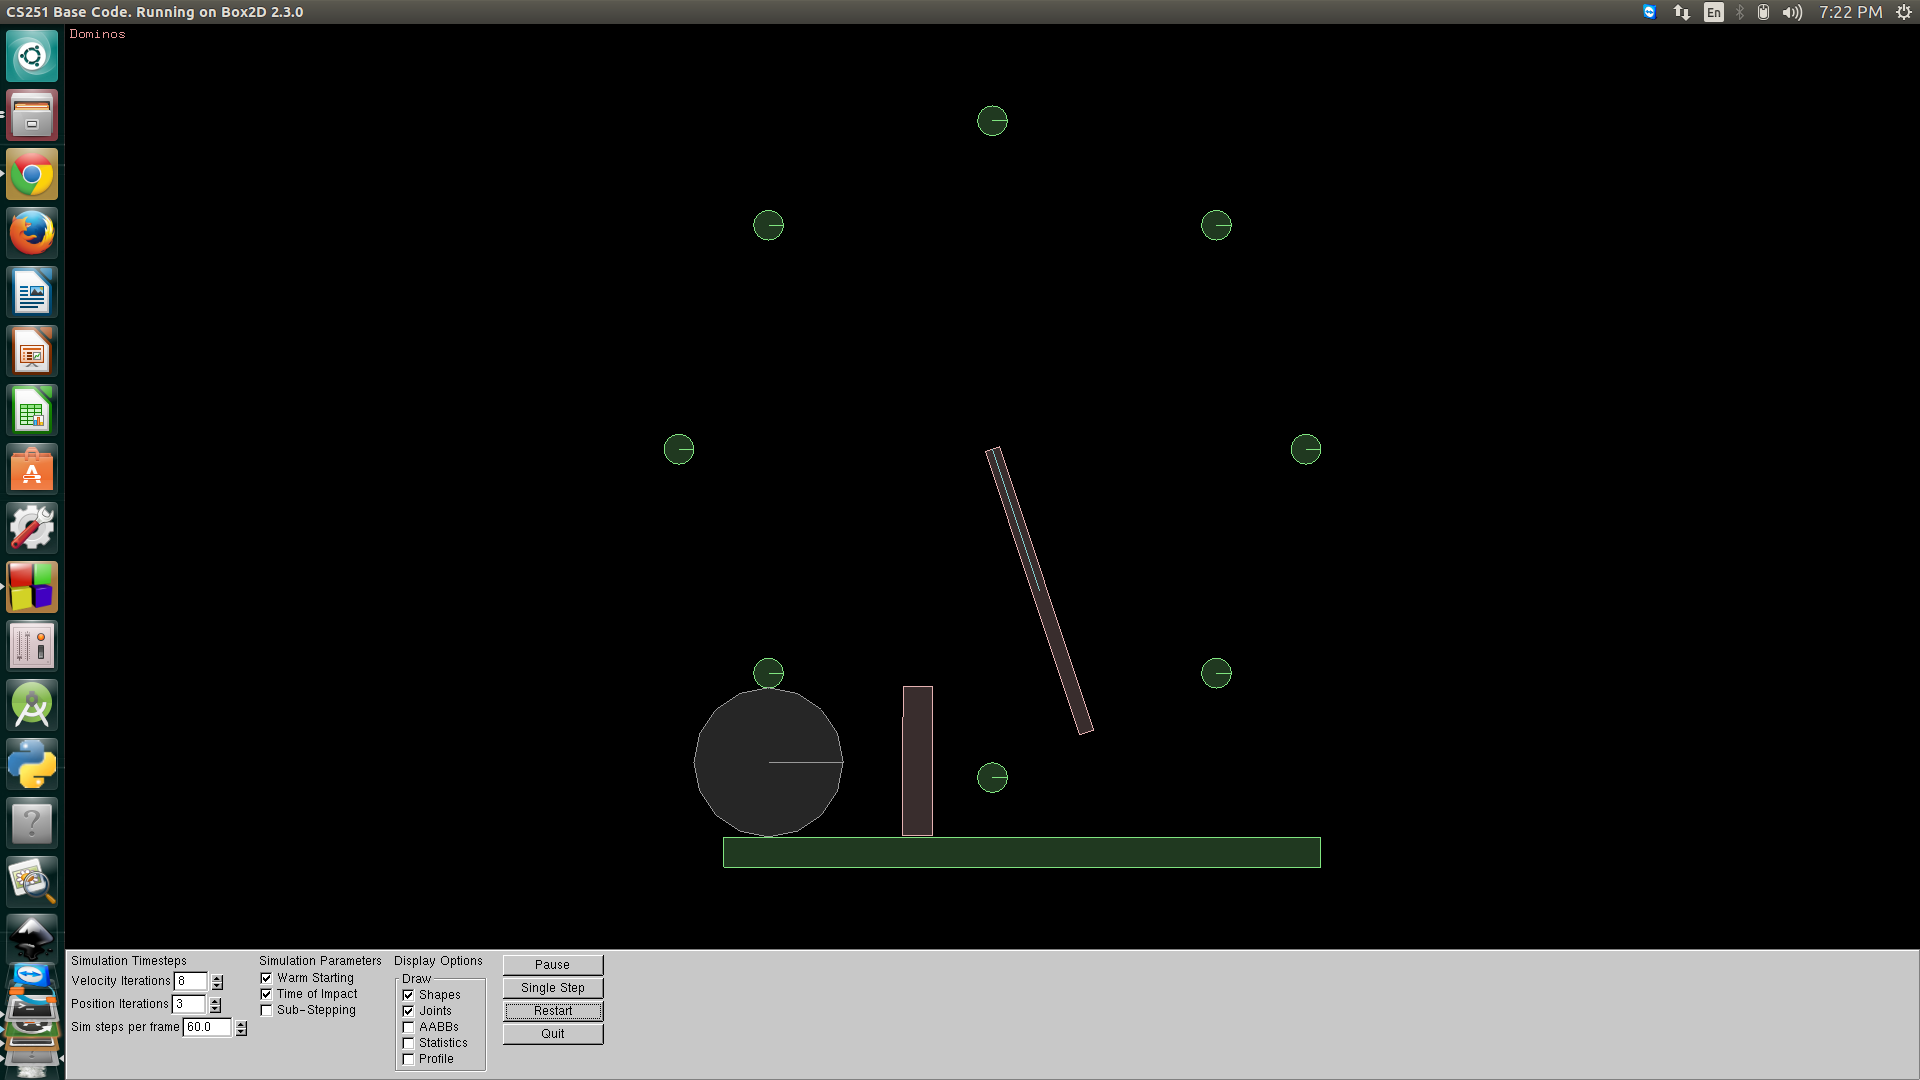
\includegraphics[scale=0.4]{project/images/clock.png}
  \caption{\textbf{call graph for clock}}
\end{figure}

\section{Seesaw and pulley}

\begin{figure}[H]
  \centering
    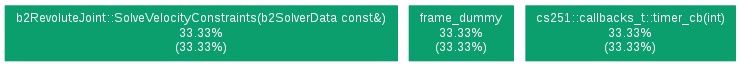
\includegraphics[scale=0.4]{project/images/seesaw.png}
  \caption{\textbf{call graph for seesaw and pulley}}
\end{figure}

\section{Curves and newton's pendulum}

\begin{figure}[H]
  \centering
    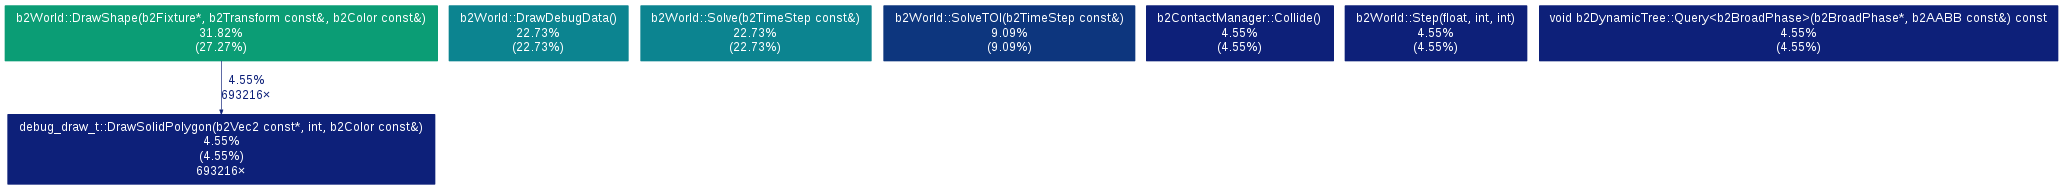
\includegraphics[scale=0.4]{project/images/curves.png}
  \caption{\textbf{call graph for curves and newton's pendulum}}
\end{figure}